%\thispagestyle{myheadings}
\section{Invited Talk: Kathleen McKeown}
\index{McKeown, Kathleen}
\begin{center}
%% --- Keynote Address ---
%% \vspace{2em}\\
%% \vfill

\begin{Large}
{\bfseries\Large ``Natural Language Applications from Fact to Fiction''}\vspace{1em}\par
\end{Large}

{\itshape Kathleen McKeown}\vspace{1em}\par
Wednesday, June 12, 2013, 9:00am -- 10:10am \vspace{1em}\\
\PlenaryLoc \\
\vspace{1em}\par
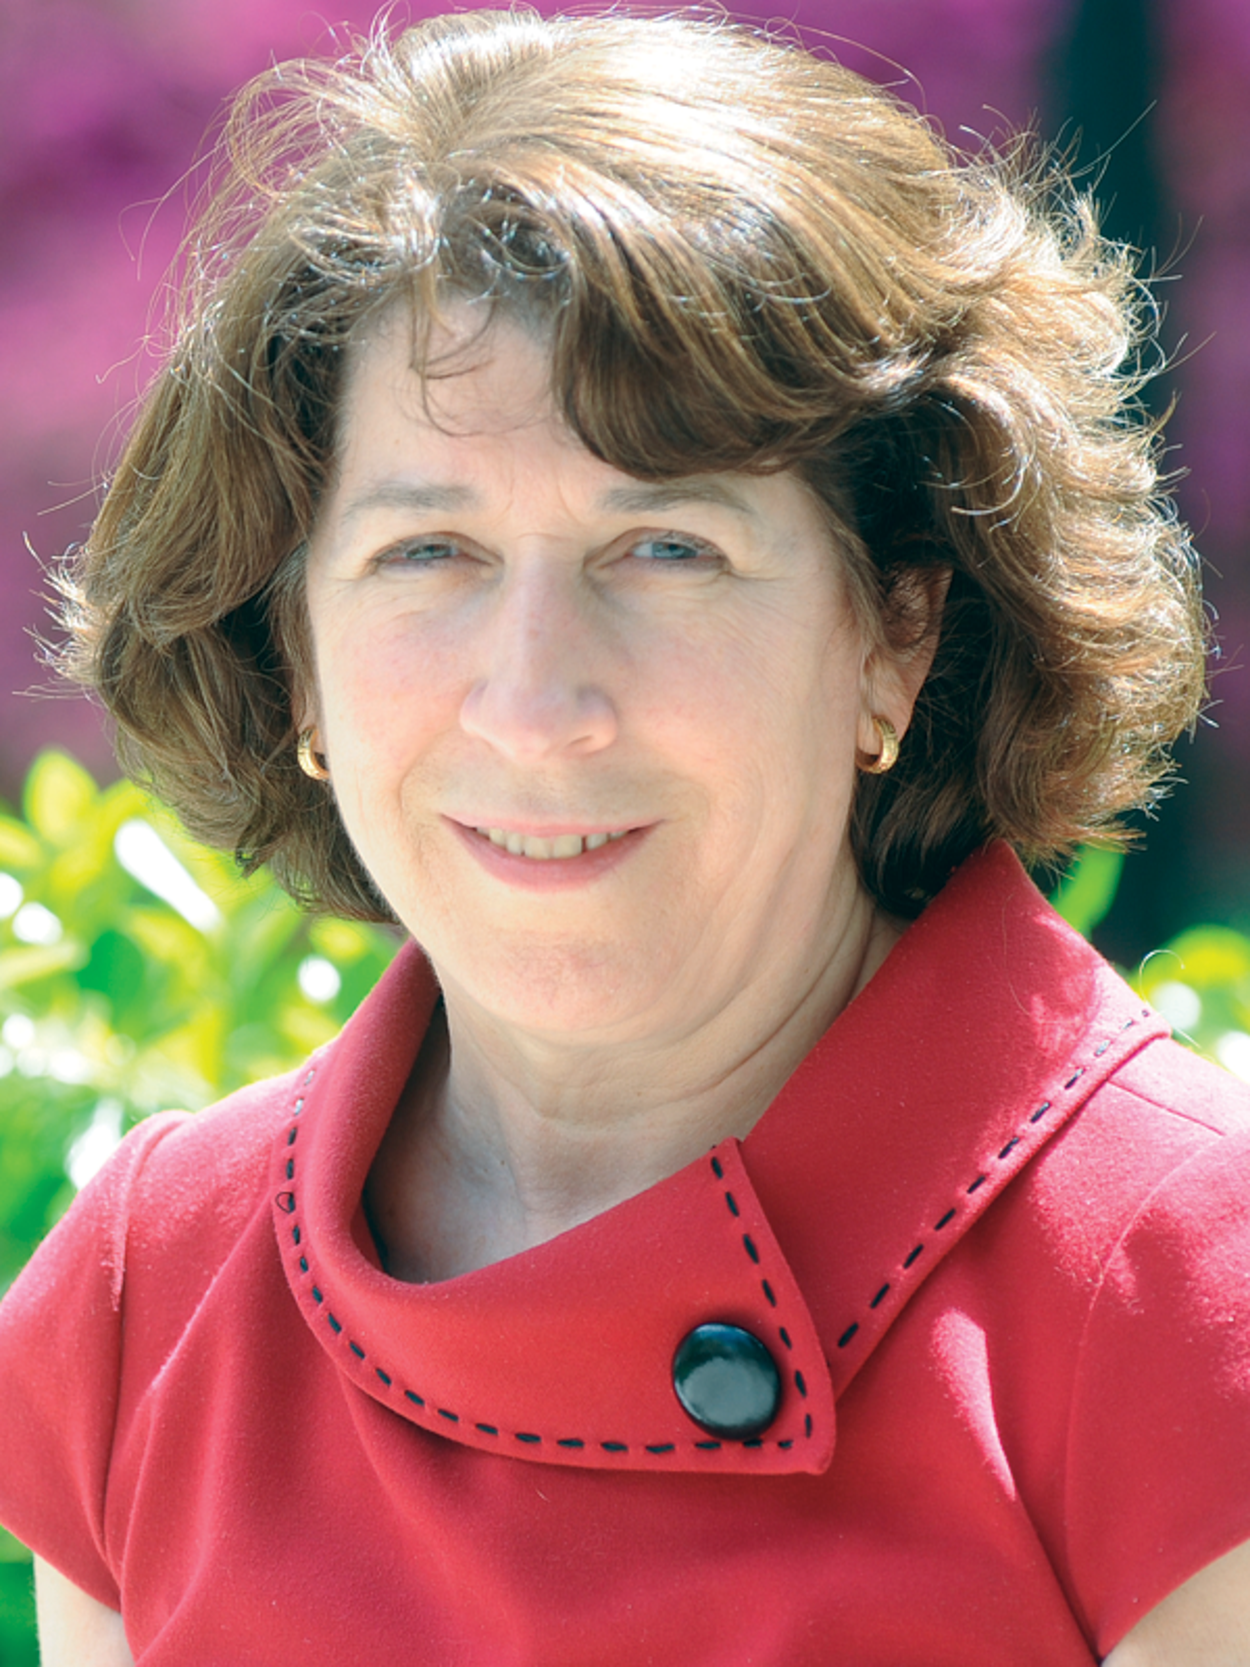
\includegraphics[height=100px]{content/day4/mckeown-headshot.pdf}
\end{center}

\noindent
{\bfseries Abstract:} Much research in the natural language field has been carried out on news, given the large amount of annotated data now available for this genre.

Certainly, the ability to analyze the facts of real world events, enabling systems to answer questions and summarize the events of the day is an important application. As research has moved to analysis of new genres, whether fact, opinion or fiction, new approaches to existing applications have arisen and opportunities for new applications have emerged. In this talk, I will present research in my group at Columbia as it has moved from news to scientific articles to online discussion forums to novels. I will touch on summarization, open-ended question answering, social influence and social networks.

\vspace{3em}\par 

\vfill
\noindent
{\bfseries Biography:} A leading scholar and researcher in the field of natural language processing,
McKeown focuses her research on big data; her interests include text summarization, question
answering, natural language generation, multimedia explanation, digital libraries, and multilingual
applications. Her research group's Columbia Newsblaster, which has been live since 2001, is an
online system that automatically tracks the day's news, and demonstrates the group's new
technologies for multi-document summarization, clustering, and text categorization, among
others. Currently, she leads a large research project involving prediction of technology emergence
from a large collection of journal articles.

McKeown joined Columbia in 1982, immediately after earning her Ph.D. from University of Pennsylvania. In 1989, she became the first woman professor in the school to receive tenure, and later the first woman to serve as a department chair (1998-2003). McKeown has received numerous honors and awards for her research and teaching. She received the National Science Foundation Presidential Young Investigator Award in 1985, and also is the recipient of a National Science Foundation Faculty Award for Women, was selected as an AAAI Fellow, a Founding Fellow of the Association for Computational Linguistics and an ACM Fellow. In 2010, she won both the Columbia Great Teacher Award—an honor bestowed by the students—and the Anita Borg Woman of Vision Award for Innovation.

McKeown served as a board member of the Computing Research Association and as secretary of the board. She was president of the Association of Computational Linguistics in 1992, vice president in 1991, and secretary treasurer for 1995-1997. She was also a member of the Executive Council of the Association for Artificial Intelligence and the co-program chair of their annual conference in 1991.

\newpage
